\chapter{مروری بر کارهای پیشین}
\newpage
‎\renewcommand{\baselinestretch}{2}\normalsize‎
\label{relatedworks}

\section{محاسبات کوانتومی توزیع شده}


محاسبات کوانتومی توزیع شده بیشتر از 15 سال مورد مطالعه قرار گرفته است\cite{ying2009algebraic}. به طور کلی مطالعاتی که در زمینه سیستم‌های کوانتومی توزیع شده انجام شده است، به دو دسته‌ی کلی تقسیم می‌گردد:
\begin{itemize}
\item
دسته‌ی اول مطالعاتی هستند که بر روی نحوی پیاده‌سازی فیزیکی این سیستم‌ها تمرکز داشته‌اند. در این مطالعات هیچ دید الگوریتمیک و بهینه‌سازی در زمینه‌ی کاهش تعداد دورنوردی‌های کوانتومی و سنتز مدارها نداشته‌اند.
\item
دسته دوم برخلاف دسته‌ی اول، شامل مطالعاتی است که به نحوه‌ی پیاده‌سازی و معماری این سیستم‌ها توجه نداشته و گامی در جهت بهینه‌سازی مدار توزیع شده با رویکرد کاهش تعداد دورنوردی‌های کوانتومی داشته‌اند. 
\end{itemize}
\section{ مطالعات دسته‌ی اول}
اولین مطالعات و پیشنهادها در مورد آن توسط گرور \cite{grover1997quantum}، کلو و بهرمن \cite{cleve1997substituting} و بعد از آن توسط کیرک در\cite{Cirac1999} بوده است. 
گرور\cite{grover1997quantum} سیستم کوانتومی توزیع شده‌ای ارائه داد که در آن ذرات در مکان‌هایی با فواصل دور از هم قرار گرفته‌اند و هر کدام  محاسبات خود را انجام داده و در صورت نیاز اطلاعات مورد نیاز را به یک ایستگاه پایه ارسال می‌نمایند. نویسندگان نشان دادند که با استفاده از محاسبات کوانتومی توزیع شده، با توجه به تعداد ذرات توزیع شده، زمان محاسبات کلی نسبتا سریعتر است. در یک مقاله دیگر، آن‌ها الگوریتمی ارائه دادند و آن‌را روی یک سیستم توزیعی که دارای هزینه‌ی محاسباتی زیادی بود، اعمال نمودند.



یپز و همکارانش \cite{yepez2001type} یک معماری برای محاسبات کوانتومی توزیع شده که دارای دو نوع ارتباطات \lr{I} و \lr{II} هستند، ارائه نمودند. آن‌ها مساله سیستم‌های کوانتومی توزیع شده را در دو نوع به این صورت تعریف نمودند: کامپیوترهای کوانتومی نوع \lr{I} از ارتباطات کوانتومی بین زیر سیستم‌ها استفاده می‌کنند. در این نوع کامپیوترها هر کیوبیت می‌تواند با هریک از کیوبیت‌های دیگر درهم‌تنیده شود. در حالی‌که در نوع \lr{II} کامپیوترهای کوانتومی از ارتباطات کلاسیک بین زیرسیستم‌ها استفاده  می‌نمایند. در این دسته از کامپیوترها، کامپیوترهای کوانتومی آرایه‌ یا شبکه‌ای از کامپیوترهای کوانتومی کوچک را در نظر گرفتند که با استفاده از کانال ارتباطی کلاسیک بهم متصل شده‌اند. بر خلاف نوع  \lr{I} که هر کیوبیت می‌توانست با هر کیوبیت دلخواه ارتباط برقرار نماید، در این نوع هر کیوبیت تنها با کیوبیت‌های نزدیک خود و در زمان کوتاه درهم‌تنیده می‌شدند. 
از آنجایی‌که تعدادی از الگوریتم‌های کوانتومی به تعداد زیادی کیوبیت (حداقل میلیون‌ها) نیاز دارند که این کیوبیت‌ها در فاصله‌ی کوتاهی از یکدیگر (حداقل در فاصله یک مولکول) و یا فقط در زمان کوتاهی (کمتر از زمان ناهمدوسی اسپین-اسپین $T_2 $) با یکدیگر در هم‌تنیده شوند\cite{yepez1998quantum} \cite{yepez1998lattice}. این چنین الگوریتم‌های کوانتومی بایستی روی آرایه و شبکه‌ای از کامپیوترهای کوانتومی با تعداد کیوبیت اندک پیاده شوند به طوری‌که گره‌ها با استفاده از یک شبکه‌ی ارتباط کلاسیک با یکدیگر در ارتباط باشند. بنابراین نیاز به کامپیوترهای کوانتومی از نوع \lr{II} احساس می‌گردد.

بیل و همکارانش \cite{Beals2013} یک سیستم کوانتومی توزیع شده ارائه دادند که در آن گره‌ها بر طبق یک گراف ابر مکعب\LTRfootnote{\lr{Hyper cube}} چیده شده، و از کیوبیت‌هایی که با فاصله زیادی از هم قرار گرفته‌اند، استفاده می‌کند. آن‌ها نشان دادند که هر مدار کوانتومی دلخواه می‌تواند با استفاده از یک مدار کوانتومی توزیع شده با گره‌های متصل شده براساس یک ابر مکعب طراحی شود.


زمانی‌که دو کیوبیت از دو سیستم کوانتومی جدا از هم بایستی با یکدیگر تعامل کنند، دو راه انتخاب مختلف وجود دارد: اول اینکه می‌توان کیوبیت از یک کامپیوتر به کامپیوتر دیگر انتقال یابد و سپس دروازه بین آن‌ها اعمال شود. دوم اینکه می‌توان از یک دروازه‌ی دورنورد شده به طور مستقیم روی کیوبیت‌ها استفاده نمود بدون اینکه کیوبیت‌ها انتقال داده شوند. نویسندگان در \cite{meter} دو نوع مختلف دورنوردی را مطرح نمودند: در نوع اول دروازه‌ها دورنوردی می‌شوند بدون اینکه کیوبیتی انتقال داده شود \lr{(telegate)}، و در نوع دوم کیوبیت‌ها انتقال داده شده و  الگوریتم روی دروازه‌های محلی که از طریق دورنوردی نمودن کیوبیت‌ها ایجاد شده‌اند، انجام می‌شوند \lr{(teledata)}. نویسندگان در \cite{gottesman1999demonstrating}  نشان دادند که مدار دورنوردی می‌تواند برای دورنوردی نمودن یک دروازه‌ی \lr{CNOT} مورد استفاده قرار گیرد. برای این کار آن‌ها نیاز به دو  زوج در هم تنیده احتیاج داشتند. اما در مطالعه‌ای که در \cite{meter} انجام شده است آن‌ها با استفاده از دروازه‌های \lr{pariaty} توانستند از یک زوج در هم‌تنیده برای دورنوردی نمودن یک دروازه استفاده نمایند. مدارهای مورد استفاده برای \lr{teledata} و \lr{telegate}  در کارآن‌ها در شکل \ref{telegateteledata} نشان داده شده است. 
مدار بالا در این شکل، مدار پروتکل دورنوردی و مدار پایین، مدار دورنوردی نمودن یک دروازه‌‌ی \lr{CNOT} می‌باشد. در این شکل، مربع با برچسب \LTRfootnote{\lr{Qubus-qubit Entanglement Protocol }}\lr{QEP} تولید کننده زوج در هم‌تنیدهِ‌ی \lr{EPR} می‌باشد. 

\begin{figure}[h]
\begin{center}
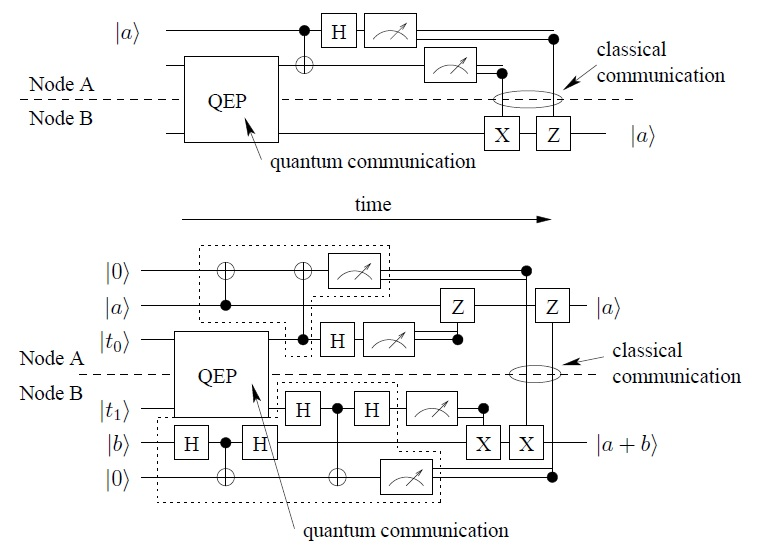
\includegraphics[scale=0.6]{telegateteledate.jpg}
\caption{مدار دورنوردی و مدار دورنوردی دروازه‌ی \lr{CNOT} \cite{meter}}
\label{telegateteledata}
\end{center}
\end{figure}

در \cite{vedral1996quantum} نویسندگان یک مدار توزیع شده با دو گره برای جمع‌کننده که با دو کیوبیت ارائه دادند و نام آن را  \LTRfootnote{\lr{ Vedral-Barenco-Ekert}}\lr{VBE} که برگرفته از نام نویسندگان بوده، قرار دادند . شکل \ref{verdal1} مدار یکنواخت آن و شکل \ref{verdal2}، مدار توزیع شده آن در دو سیستم را نشان می‌دهد. در این شکل، کیوبیت $\ket{C_0}$ از گره‌ی \lr{A} به گره‌ی \lr{B} منتقل می‌شود. این کیوبیت که برای محاسبات در گره‌ی \lr{B} مورد استفاده قرار می‌گیرد، به گره‌ی \lr{A} از طریق مدار دورنوردی مشابه با قبل منتقل می‌گردد. همچنین دو کیوبیت $\ket{t_0}$ و $\ket{t_1} $ به عنوان کیوبیت‌های گیرنده و فرستنده مورد استفاده قرار گرفته‌اند.  

\begin{figure}[h]
\begin{center}
\includegraphics[scale=0.6]{meter.jpg}
\caption{مدار یکنواخت جمع کننده\cite{meter}}
\label{verdal1}
\end{center}
\end{figure}

\begin{figure}[h]
\begin{center}
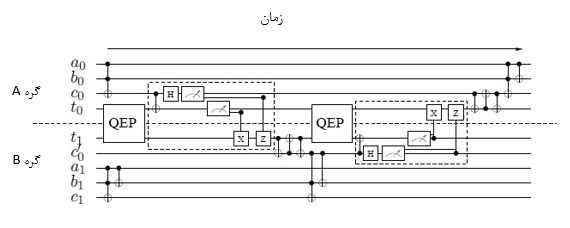
\includegraphics[scale=0.7]{dimeter.jpg}
\caption{ در این مدار مستطیل\lr{QEP} تولید کننده زوج در هم تنیده \lr{EPR} بوده و مداری که با خط چین نشان داده شده است بیانگر مدار دورنوردی است.}
\label{verdal2}
\end{center}
\end{figure}

نویسندگان در \cite{meter} یک مدار جمع کننده \lr{VBE} بزرگتر طراحی نمودند و دو روش \lr{telegate} و \lr{teledata} را با یکدیگر مقایسه نمودند. آن‌ها نشان دادند که روش \lr{teledata} نسبت به \lr{telegate}  دارای کارایی بهتری است. شکل \ref{meter} مدار مورد استفاده‌ی آن‌ها برای یک جمع کننده بزرگتر را نشان می‌دهد. نویسندگان چند مساله را در کار خود در زمینه‌‌ی نسخه‌ی توزیعی مدارهای کوانتومی بررسی نکردند. اولین ایده، در رابطه با یافتن کمترین تعداد کیوبیت برای دورنوردی بود. ایده آن‌ها برای مدارهای کوچک انجام شد. به‌هرحال برای مدارها با اندازه‌ی بزرگ، یافتن تعداد کیوبیت‌ها که منجر به حداقل هزینه‌ی کوانتومی گردد، یک چالش بزرگ است. 
%ایده‌ی دیگر که توسط ون متر در \cite{meter} بیان شده است، در این مورد بود که اگر برخی دروازه‌های پشت سرهم که در گره هدف وجود داشته باشند، که از کیوبیت دورنوردی شده در یکی از ورودی‌های خود استفاده می‌کنند، در این صورت کیوبیت دورنوردی شده می‌تواند بصورت پشت سرهم در این دو دروازه در نود مقصد مورد استفاده قرار گیرد. اما همیشه این مورد صحیح نمی‌باشد. گاهی اوقات کیوبیتی که دورنوردی شده است، در سمت مبدا مورد نیاز است و بایستی در میانه کار به سمت مبدا خود برگردد که این منجر به افزایش هزینه سیستم می‌گردد.


این مدار طوری طراحی شده است تا بتوان تعداد مورد استفاده از \lr{teledat} و \lr{telegate} را نشان دهد. در این شکل خطوط خط چین قرمز بیانگر \lr{teledata} و خطوط خط چین آبی جایی است که مدار از \lr{telegate} استفاده نموده است. همانطور که این شکل نشان می‌دهد، تعداد دفعاتی که \lr{telegate} رخ داده است، از تعداد دفعاتی که \lr{teledata} رخ داده است، بیشتر است. 


\begin{figure}[h]
\begin{center}
\includegraphics[scale=0.7]{vbelarge.jpg}
\caption{مقايسه تعداد \lr{telegate}  و تعداد \lr{teledata} در مدار \lr{VBE} مورد نظر. خطوط قرمز خط چين بيانگر \lr{teledata} و خطوط آبي خط چين بيانگر \lr{telegate} مي‌باشد.}
\label{meter}
\end{center}
\end{figure}
 همانطور که پیشتر بیان شد، ایجاد در هم‌تنیدگی کوانتومی بین دو کیوبیت که در فاصله‌ی زیادی از هم قرار گرفته‌اند، مرحله‌ای اساسی در پردازش اطلاعات کوانتومی است که این عمل به دلیل بعد مسافتی برای سیستم هزینه‌بر می‌باشد. استرلسا و و همکارانش در  \cite{streltsov} بهترین راه برای درهم‌تنیدگی و با کمترین هزینه برای ارسال حالت‌های درهم‌تنیده در فواصل دور را مطرح کردند. آن‌ها نشان دادند که این هزینه ذاتا کوانتومی بوده و  با استفاده از هم‌بستگی کوانتومی مشخص می‌گردد. نتایج آن‌ها نشان داد که پروتکل پیشنهادی برای توزیع در هم‌تنیدگی به لحاظ هزینه بهینه بوده و هم‌بستگی کوانتومی یک منبع ضروری برای آن است.
 
%استفاده از در اکثر پروتکل‌های توزیعی، تعداد درهم‌تنیدگی فرستاده شده در سیستم  توزیعی نمی‌تواند بزرگتر ازکل هزینه درهم‌تنیدگی برای رفت و برگشت یک ذره باشد.
يكي از كاربردهاي اصلي و اساسي محاسبات كوانتومي توزيع شده، استفاده آن در اينترنت كوانتومي است. در \cite{caleffi2018quantum} نویسندگان به افزایش نمایی سرعت محاسبات کوانتومی اشاره نمودند که از طریق ارتباطات کامپیوترهای کوانتومی با استفاده از اینترنت کوانتومی بدست آمده است. یکی از کاربردهای سیستم‌های کوانتومی توزیع شده اینترنت کوانتومی است. اینترنت کوانتومی شبکه‌ای از دستگاه‌های کوانتومی هستندکه قادرند تا حالات کوانتومی را بین دستگاه‌های از راه دور به اشتراک بگذارند، بدون این‌که مزایای آن کاهش یابد. همچنین آن‌هادر مطالعه‌ی خود بیان نمودند که استفاده از اینترنت کوانتومی با محدودیت‌هایی مانند عدم کپی‌برداری، درهم‌تنیدگی و دورنوردی کوانتومی مواجه است، در حالی‌که در شبکه‌های کلاسیک این چالش‌ها موجود نمی‌باشند. بنابراین آن‌ها در مطالعه‌ی خود به بررسی این چالش‌ها پرداختند. %در مدل محاسباتی استاندارد در یک دستگاه کوانتومی، تعامل بین هر دو جفت کیوبیت فیزیکی امکان پذیر است. در حالی که در یک دستگاه کوانتومی واقعی محدودیت‌هایی در ارتباطات فیزیکی کیوبیت‌ها وجود دارد. قدرت محاسباتی یک کامپیوتر کوانتومی به تعداد کیوبیت‌هایی که در آن نهفته است، وابسته است. اما پیشرفت تکنولوژی‌های کوانتومی محدود به تعداد اعداد دو رقمی است. 
‌آن‌ها بیان نمودند که چگونه می‌‌توان کیوبیت‌های یک سیستم را افزایش داد تا بتوان به برتری کوانتومی دست یافت؟ پاسخ آن‌ها این بود تا کامپیوترهای کوانتومی از طریق اینترنت کوانتومی با یکدیگر در تعامل باشند. برای مثال دو سیستم کوانتومی مجزای ده کیوبیتی می‌توانند $2^{10}$ حالت کوانتومی را ارائه دهند و بنابراین این دو سیستم $2.2^{10}$ حالت را نشان دهند. اما اگر از طریق اینترنت کوانتومی با یکدیگر تعامل داشته باشند، می‌تواند
 $2^{18}$ حالت را نشان دهند. شکل \ref{speedup}  میزان رشد افزایش محاسبات کوانتومی در برابر افزایش تعداد سیستم‌ها را نشان می دهد.
\begin{figure}[h]
\begin{center}
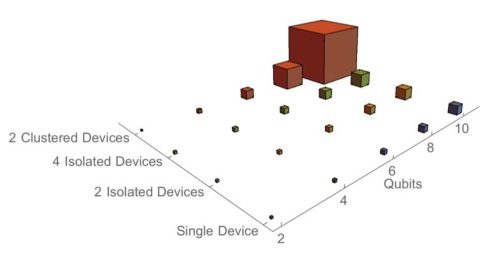
\includegraphics[scale=0.7]{speedup.jpg}
\caption{سرعت محاسبات ابری کوانتومی- حتی در مورد دستگاه‌های کوچک کوانتومی، دو  دستگاه کوانتومی خوشه شده می‌تواند سرعت نمایی  در مقایسه با یک دستگاه مجزا فراهم نماید.}
\label{speedup}
\end{center}
\end{figure}


در \cite{cacciapuoti2019quantum} نویسندگان به مطالعه و بررسی چالش‌های موجود در اینترنت کوانتومی پرداختند. همان‌طور که از طریق اینترنت کنونی می‌توان اطلاعات را منتقل نمود، از طریق اینترنت کوانتومی نیز می‌توان ارتباطات مورد نیاز را انجام داد. برای مثال نمونه‌ای از ارتباطات کوانتومی، در توزیع کلید کوانتومی \lr{(QKD)} \LTRfootnote{\lr{Quantum Key Distribution}} می‌باشد. \lr{QKD} یک پروتکل رمزنگاری است که می‌تواند بین دو ذره، یک کلید تصادفی مشترک با استفاده از قوانین مکانیک کوانتوم  ایجاد نماید. همچنین آن‌ها بیان نمودند که با استفاده از اینترنت کوانتومی می‌توان حالات کوانتومی را بین گره‌های از راه دور به اشتراک گذاشت. اما همان‌طور که قبلا بیان شد، یک کیوبیت با محدودیت‌هایی مانند کپی برداری و اندازه‌گیری مواجه است. گرچه یک فوتون می‌تواند یک کیوبیت را رمز نماید\LTRfootnote{\lr{Encode}}  و به گره‌های راه دور (از طریق فیبر نوری) ارسال شود، اما چنانچه فوتون ارسال شده در معرض نویز قرار گیرد، اطلاعات کوانتومی ازبین می‌رود و از آنجایی که اطلاعات کوانتومی بر طبق تئوری عدم کپی، قابلیت کپی برداری ندارد، بنابراین انتقال مستقیم اطلاعات کوانتومی از طریق فوتون امکان پذیر نمی‌باشد و بایستی از پروتکل دورنوردی استفاده نمود. 





مطالعه‌ی دیگر جهت پیاده‌سازی توزیعی مدارهای کوانتومی در \cite{yimsiriwattana} آمده است. نویسندگان بیان نمودند که می‌توانند کامپیوترهای کوانتومی با ظرفیت اندک را با یکدیگر ترکیب نموده تا کامپیوتر کوانتومی در مقیاس بزرگ شبیه‌سازی نمایند. آن‌ها الگوریتم کوانتومی تجزیه‌ی شور را روی یک شبکه کوانتومی توزیع شده پیاده‌سازی نمودند. آن‌ها در روش خود از در هم‌تنیدگی کوانتومی جهت پیاده‌سازی دروازه‌های غیر محلی بین دو یا تعداد بیشتری کامپیوتر کوانتومی استفاده نمودند و نشان دادند برای پیاده‌سازی و اجرای این دروازه‌های محلی نیاز به تعداد زیادی دروازه‌ دارند که تعداد این دروازه‌ها دارای مرتبه زمانی خطی بود. ایسرت و همکارانش در \cite{eisert2000optimal} حداقل تعداد دروازه‌های مورد نیاز برای پیاده سازی دروازه‌های غیر محلی به صورت محلی را پیش بینی نمودند و از آنجایی که یک دروازه‌ی  \lr{CNOT} با تمام دروازه‌های تک کیوبیتی یک مجموعه‌ی مرجع است، بنابراین با استفاده از دروازه‌های غیر محلی \lr{CNOT} می‌توان پیاده‌سازی توزیع شده هر انتقال یکانی \LTRfootnote{\lr{Unitary transformation}} را انجام داد. برای پیاده‌سازی یک دروازه‌ی غیر محلی \lr{CNOT} یک جفت زوج در هم‌تنیده و دو بیت کلاسیک لازم و کافی است \cite{eisert2000optimal}. آن‌ها از دو عملگر مهم بنام \lr{cat-entangler} و \lr{cat-disentangler} که توسط آنوکا و همکارانش \cite{yimsiriwattana2004generalized} ارائه گردید، جهت پیاده‌سازی عملگرهای غیرمحلی مانند دروازه‌های سراسری \lr{CNOT} و پروتکل دورنوردی کوانتومی استفاده نمودند. شکل \ref{fig81} این دو عملگر را نشان می‌دهد. 
\begin{figure}
\centering
\includegraphics[scale=0.6]{catdiscat.jpg}
\caption{ \lr{A}. مدار عملگر \lr{cat-entangle}.\lr{B}: مدار عملگر \lr{cat-disentangler}  }
  \label{fig81}
%\end{center}
\end{figure}


در این شکل، خط چین‌ها بیانگر نتیجه‌ی حاصل از عملگر اندازه گیری بوده که برای دروازه‌ی \lr{X} بکار می‌رود. همچنین دروازه‌ی \lr{Z} در مدار سمت راست، با عملگر یای انحصاری سه بیت کلاسیک اندازه گیری شده در مدار سمت چپ کنترل می‌شود.
نویسندگان نشان دادند، برای پیاده‌سازی یک دروازه‌ی  \lr{CNOT} بایستی یک جفت درهم‌تنیده، بین دو کامپیوتر ایجاد گردد. سپس یک \lr{cat-entangler} جهت انتقال کیوبیت کنترلی $\alpha\ket{0}+\beta\ket{1}$ و  تبدیل حالت زوج در هم تنیده‌ی $\frac{1}{\sqrt{2}}(\ket{00}+\ket{11})$ به حالت $\alpha\ket{00}+\beta\ket{11}$ (به نام \lr{cat-like}) اعمال می‌گردد. این حالت به کامپیوترها اجازه می دهد تا کیوبیت کنترلی را بین خود به اشتراک بگذارند. درنتیجه، هر کامپیوتر می‌توانند از طریق حالت \lr{cat-like}، از کیوبیت به اشتراک گذاشته شده به عنوان کیوبیت کنترلی محلی استفاده نماید.
پس از آن، \lr{cat-disentangler} جهت جداسازی کیوبیت کنترلی از حالت \lr{cat-like} اعمال می‌گردد. در نهایت کیوبیت‌های کانال با استفاده از اطلاعات کلاسیکی از عملگر اندازه‌گیری برای کنترل نمودن دروازه‌ی \lr{X} بدست آمده است، بازنشانی\LTRfootnote{\lr{Reset}} می‌شوند. سربار اضافی این مدار توزیعی در تعداد مدارهای دورنوردی بوده است و آن‌ها هیچ تلاشی برای کاهش این تعداد نداشته‌اند. شکل \ref{figcnot} یک مدار \lr{CNOT} غیرمحلی را نشان می‌دهد. 
\begin{figure}[h]
\centering
\includegraphics[scale=0.6]{nonlocalcnot.jpg}
\caption{ مدار \lr{CNOT} غیر محلی  }
  \label{figcnot}
%\end{center}
\end{figure}

برای دورنوردی نمودن یک کیوبیت ناشناخته از کامپیوتر کوانتومی \lr{A} به کامپیوتر \lr{B}، یک زوج در هم‌تنیده بین دو کامپیوتر ایجاد می گردد. سپس با استفاده از عملگر \lr{cat-entangler}، حالت\lr{cat-like} از یک کیوبیت ناشناخته و جفت در هم تنیده ایجاد می‌شود. سپس با اعمال عملگر \lr{cat-disentangler} عمل جداسازی کیوبیت ناشناخته از حالت \lr{cat-like} به کامپیوتر \lr{B} انجام می‌شود. در نهایت عمل \lr{swap} بین کیوبیت ناشناخته با کیوبیت $\ket{0}$ انجام می‌گردد. مدار دورنوردی مورد استفاده در کار آن‌ها در شکل \ref{teleshor} نشان داده شده است.
\begin{figure}[h]
\centering
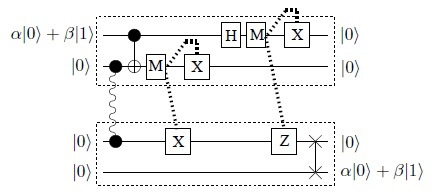
\includegraphics[scale=0.6]{teleshor.jpg}
\caption{مدار دورنوردی مورد استفاده  }
  \label{teleshor}
%\end{center}
\end{figure}

هزینه‌ی ارتباطات کلاسیک در محاسبات کوانتومی موضوع مورد مطالعه در \cite{lo2000classical} بوده است. نویسندگان نشان دادند که در یک دورنوردی دو مرحله‌ای، هر مرحله نیاز به یک بیت برای ارتباطات کلاسیک دارد و در حالت کلی برای حالتی با \lr{N} بعد، \lr{$2\log_{2}N$} بیت ارتباطات کلاسیک جهت آماده‌سازی از راه دور داریم. این هزینه نسبت به هزینه دورنوردی معمولی متفاوت است. (در دورنوردی معمولی حالت دقیق یک کیوبیت در دریافت کننده برای فرستنده کاملا شناخته شده است.)

یینگ و همکارانش \cite{ying2009algebraic} برخی تعاریف برای سیستم‌های محاسباتی کوانتومی توزیع شده ارائه دادند. آن‌ها بیان نمودند که یکی از روش‌های مناسب برای نمایش مدارهای کوانتومی نمایش آن به صورت گراف است که می‌تواند به فهم و شناخت مدار کمک نماید. از دیگر روش‌های نمایش مدارهای کوانتومی نمایش آن به صورت یک عبارت دودودیی و جبری است و از مزایای آن اعمال محاسبات جبری در آن است. آن‌ها یک زبان جبری برای توصیف چگونگی نمایش  محاسبات کوانتومی توزیع شده برای مدارهای کوانتومی ارائه دادند.
\section{مطالعات دسته دوم}
در این دسته از مطالعات، نویسندگان گامی در جهت طراحی سیستم‌های کوانتومی با هدف کاهش تعداد دورنوردی‌های کوانتومی توزیع شده برداشته‌اند. در ادامه به بررسی تعدادی از آن‌ها پرداخته شده است.

 پابلو و همکارانش \cite{Pablo} الگوریتمی خودکار جهت توزیع نمودن مدار کوانتومی به چندین زیر سیستم ارائه نمودند. معماری محاسبات کوانتومی توزیع شده در چندین ویژگی مشترک هستند \cite{van2016path}:
\begin{itemize}
\item
واحدهای پردازش کوانتومی یا \lr{(QPU)}: هر واحد شامل تعدادی کیوبیت است و می‌توان دروازه‌های کوانتومی را روی آن‌ها اعمال نمود. کیوبیت‌های هر واحد بایستی قادر باشد تا داده‌های ورودی هر برنامه را در خود نگه داشته و خروجی را از طریق اندازه‌گیری\LTRfootnote{\lr{Measurement}} از آن‌ها بخوانند.

\item
شبکه ارتباطی کلاسیک\LTRfootnote{\lr{Classical communication network}}: هر واحد \lr{QPU} نیاز دارد تا یک پیام کلاسیک را هنگام اندازه‌گیری کیوبیت‌هایش از طریق کانال کلاسیک ارسال نماید و یا اینکه در هنگام خطا پیامی دریافت نماید. بنابراین نیاز به یک کانال ارتباطی کلاسیک می‌باشد.
\item
سخت افزار تولید \LTRfootnote{\lr{Entangle bit}}\lr{ebit}: هر \lr{ebit} شامل حالت درهم‌تنیده دو کیوبیت است که هر کیوبیت روی \lr{QPU} های متفاوتی ذخیره شده‌اند و به هر کدام از  آن‌ها \lr{ebit halves} گفته می‌شود. هر \lr{ebit} شامل اطلاعات یک کیوبیت برای انتقال آن از یک واحد به واحد دیگر است. بسته به تکنولوژی و  نویزی‌بودن کانال کوانتومی، هر واحد خود می‌تواند دارای سخت افزاری جهت تولید \lr{ebit} باشد و یا اینکه یک دستگاه مجزا مرکزی وجود داشته باشد که خود تولید کننده \lr{ebit} باشد\cite{bennett1996mixed}. چالش اصلی در یک سیستم کوانتومی توزیع شده، همان تولید کننده \lr{ebit} است که نسبت به ارتباطات کلاسیک  و هر عمل منطقی گران‌تر است.
\item
فضای ذخیره سازی \lr{ebit}: این فضا بیانگر فضای مورد نیاز در جهت ذخیره‌سازی \lr{ebit} می‌باشد.
\end{itemize}
در هر سیستم کوانتومی توزیعی، سازشی بین \lr{ebit}  و منابع تخصیص داده شده برای آماده‌سازی آن وجود دارد\cite{bennett1996purification}. خوشبختانه ایجاد یک سیستم کوانتومی توزیع شده و کارآمد با استفاده از \lr{ebit} هایی که شامل نویز هستد، کاری امکان‌پذیر است\cite{Cirac1999}.

آن‌ها مساله‌ی توزیع مدارهای کوانتومی را به مساله‌ی افرازبندی ابرگراف\LTRfootnote{\lr{Hypergraph}} کاهش دادند و با استفاده از الگوریتم افراز‌بندی ابرگراف که در \cite{akhremtsev2017} ارائه شده است، مدار را در چند زیر سیستم توزیع نمودند. ایده‌ی اصلی الگوریتم پیشنهادی آن‌ها در این بود زمانی که دو دروازه‌ی سراسری پشت سرهم وجود دارند که دارای کیوبیت کنترلی مشترک هستند، با دورنوردی کیوبیت کنترلی اولین دروازه، دروازه‌ی دوم نیز اجرا شود. آن‌ها در کار خود از دو مدار \lr{cat-entangler} و \lr{cat-disentangler} تعریف شده در\cite{yimsiriwattana} استفاده نمودند. شکل \ref{9} چگونگی توزیع نمودن دو دروازه سراسری پشت سرهم که در یک کیوبیت مشترک هستند، نشان می‌دهد. دروازه‌های $\alpha$ و $\beta$ دو دروازه‌ی سراسری پشت سرهم بوده و دارای کیوبیت کنترلی یکسان \lr{C} می‌باشند. برای اجرای دروازه‌ی $\alpha$ کیوبیت \lr{C} از افراز دوم به افراز اول دورنوردی می‌شود. از آنجایی که دروازه‌ی $\beta$ نیز دارای کیوبیت کنترلی \lr{C} می‌باشد. بنابراین با دورنوردی نمودن کیوبیت \lr{C} این دو دروازه همزمان می‌توانند اجرا شوند. 
\begin{figure}[h]
\begin{center}
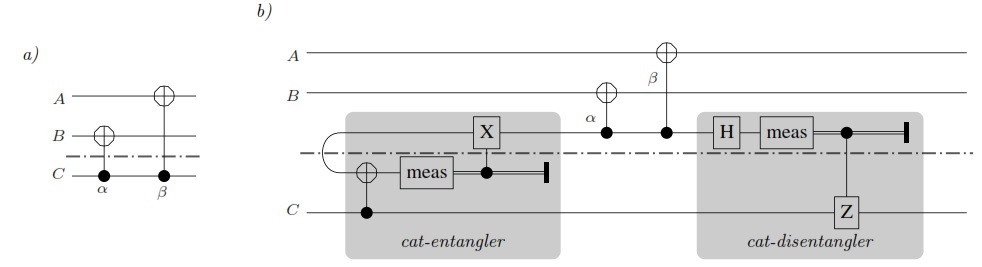
\includegraphics[scale=0.6]{fig9.jpg}
\caption{پیاده‌سازی دو دروازه‌ی پشت سرهم با یک کیوبیت مشترک \cite{Pablo}}
\label{9}
\end{center}
\end{figure}


همانطور که در بالا اشاره گردید، الگوریتم آن‌ها یک مدار کوانتومی را به یک ابرگراف کاهش می‌داد. جدول \ref{pabelo} چگونگی کاهش این مساله را به مساله‌ی افرازبندی ابرگراف نشان می‌دهد. برای این کار، آن‌ها رئوس ابرگراف را به عنوان کیوبیت‌ها در نظر گرفتند. همچنین ابریال‌ها در مساله آن‌ها گروهی از دروازه‌های \lr{CZ} که پشت سر هم بود، در نظر گرفته شد. توزیع مدار همان مفهوم افرازها در ابرگراف و واحدهای کوانتومی همان بلوک‌ها در ابرگراف بود. هدف آن‌ها در این مساله کاهش تعداد دورنوردی‌های کوانتومی با رویکرد توزیع متوازن کیوبیت‌ها بود. نمونه‌ای از این کاهش در شکل \ref{reduct} نشان داده شده است. 
\begin {table}[h]
\begin{center}
\caption{چگونگی کاهش مساله‌ی توزیع مدار کوانتومی به افرازبندی ابرگراف \cite{Pablo}}
\label{pabelo}
 \begin{tabular}{c|c}

افرازبندی ابرگراف& توزیع مدار\\
\hline
&\\
\lr{Vertices}&\lr{Wires(qubits)}\\
\lr{Hyperedges}&\lr{Groups of CZs}\\
\lr{Partition}&\lr{Distribution}\\
\lr{Blocks}&\lr{QPUs}\\
\lr{Load-balance}&\lr{Load-balance}\\
\lr{Fewest cuts}&\lr{Fewest ebits used}\\
\end{tabular}
\end{center}
\end{table}

\begin{figure}[h]
\centering     
\subfigure[مدار کوانتومی ارائه شده با پنج دروازه و چهار کیوبیت]{\label{fig:a}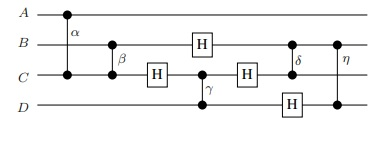
\includegraphics[width=70mm]{pabelo2}}
\subfigure[چگونگی تبدیل مدار\ref{fig:a} به ابرگراف]{\label{fig:b}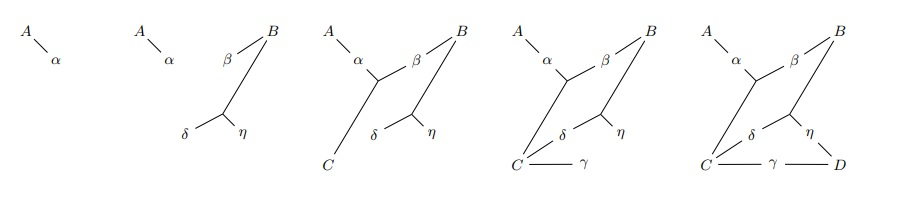
\includegraphics[width=90mm]{pabelo1}}
\caption{چگونگی کاهش مدار کوانتومی به ابرگراف در \cite{Pablo}}
\label{reduct}
\end{figure}


محدودیت کار آن‌ها در این بود که آن‌ها جهت کاهش تعداد دورنوردی های کوانتومی، تنها دروازه‌هایی سراسری \lr{CZ} پشت سرهم که در کیوبیت کنترلی مشترک بودند، در نظرگرفته و آن‌ها را با یک دورنوردی کوانتومی اجرا نموده و حالات دیگر را در نظر نگرفتند. 
در انتها الگوریتم پیشنهادی خود را روی پنج نمونه مدار کوانتومی تست نمودند. 

زمردی و همکارانش\cite{Zomorodi} الگوریتمی جهت کاهش تعداد دورنوردی‌های مورد نیاز در یک مدار کوانتومی ارائه دادند. در این الگوریتم از دو سیستم کوانتومی مجزا که در فواصل طولانی از همدیگر قرار گرفته بودند، استفاده شد. آن‌ها دو سیستم کوانتومی در نظر گرفته و کیوبیت‌ها را به طوری مساوی در آن توزیع نمودند. همچنین در کار خود نشان دادند چنانچه یکی از کیوبیت‌های یک دروازه سراسری از زیر سیستم مبدا به زیر سیستم مقصد دورنوردی شود، می‌تواند توسط دیگر دروازه‌های سراسری مورد استفاده قرار گیرد و سپس به زیر سیستم مبدا خود باز گردد. برای هر دروازه برچسبی به نام $l$ در نظر گرفته شده که دارای مقدار 0 یا 1 می‌باشد. چنانچه این برچسب دارای مقداری 0 باشد، به معنای این است که این دروازه بایستی در افراز 0 اجرا شده و چنانچه دارای مقدار 1 باشد، به این معناست که این دروازه بایستی در افراز 1 اجرا گردد. آن‌‌ها در کار خود لیستی از دروازه‌ها به نام $\mathcal{G}$ در نظر گرفتند. سپس از ابتدای لیست هر دروازه را بررسی نموده، در صورتی‌که دروازه‌ی مورد نظر محلی بوده از لیست $\mathcal{G}$ حذف شده درغیر این صورت تصمیم به ارسال یکی از کیوبیت‌های آن می‌گردد. در الگوریتم اصلی، آن‌ها از دو تابع به نام‌های \lr{Non-Execute} و \lr{Non-Commute} استفاده نمودند که هر کدام از آن‌ها به صورت زیر تعریف گردید:

\begin{itemize}
\item
تابع \lr{Non-Execute}: این تابع دو دروازه‌ی $g$ و $g^{'}$ را به عنوان ورودی دریافت می‌کند. این تابع مقدار \lr{True} برگردانده، در صورتی که کیوبیت دورنورد شده‌ی دروازه‌ی $g$، بنا به یکی از سه حالت ذکر شده در زیر، بایستی به افراز مبدا خود باز گردد و بعد از آن دروازه‌ی $g^{'}$  اجرا شود. در غیر این صورت این تابع مقدار \lr{False} باز می‌گرداند. این سه حالت عبارت‌اند از:

\begin{itemize}
\item
دروازه‌ی $g^{'}$ یک دروازه‌ی محلی است که یکی از کیوبیت‌های آن با کیوبیت‌ دورنوردی شده‌ی $g$ یکی است.
\item
دروازه‌ی  $g^{'}$ یک دروازه‌ی سراسری با برچسبی متفاوت با دروازه‌ی $g$ باشد.
\item
دروازه‌ی $g^{'}$ یک دروازه‌ی سراسری با برچسبی یکسان با دروازه‌ی $g$ است اما جهت اجرا نیاز به دورنوردی دیگری دارد.
\end{itemize}
\item
تابع \lr{Non-Commute}: این تابع دو دروازه را به عنوان ورودی دریافت می‌نماید. در صورتی‌که این دو دروازه بتوانند با یکدیگر جابجا شوند، این تابع مقداری \lr{True}، در غیر این صورت مقداری \lr{False} برمی گرداند. 
\end{itemize}


آن‌ها بیان نمودند که اگر سیستم توزیع شده دارای  $n$ دروازه‌ی سراسری باشد، تعداد $2^{n}$ پیکربندی ممکن برای انجام دورنوردی‌های لازم بر روی دو زیرسیستم کوانتومی وجود داشته و از بین این حالات، حالتی که منجر به یافتن کمترین تعداد دورنوردی‌ها در بین تمام پیکربندی‌های ممکن می‌گردد، به عنوان حالت بهینه در نظر گرفته می‌شود. آن‌ها تمام پیکربندی‌های ممکن از اجرای دروازه‌ها را بررسی نمودند و نشان دادند که الگوریتم ارائه شده‌ی آن‌ها دارای زمان نمایی است. محدودیت الگوریتم آن‌ها این بود که دارای زمان اجرای نمایی بود. همچنین الگوریتم آن‌ها برای دو افراز ثابت بوده و برای چند افراز بررسی نگردید.

در کار دیگری از زمردی و همکارانش \cite{ZomorodiE}، الگوریتمی تکاملی ارائه گردید تا مساله‌ی کاهش تعداد دورنوردی‌ها را به صورت کاراتر حل نمایند. آن‌ها در کار خود یک الگوریتم ژنتیک ارائه دادند و دو پرسش را مطرح نمودند:

1- زمان اجرای یک دروازه‌ی سراسری \lr{CNOT}، کدام کیوبیت آن (کنترل یا هدف) بایستی دورنوردی شود و آیا این انتخاب تاثیری بر تعداد دورنوردی‌ها دارد؟

2- سوال دیگر آن‌ها این بود که چه زمانی بایستی کیوبیت دورنورد شده به مبدا اولیه خود برگردد؟ و آیا اینکه همانند سوال قبل این انتخاب بر تعداد دورنوردی‌ها تاثیری می‌گذارد یا خیر؟

نویسندگان در کار خود با استفاده از الگوریتم ژنتیک روشی ابتکاری پیشنهاد دادند که بتواند بهترین پیکربندی از دروازه‌های سراسری را با هدف کاهش تعداد دورنوردی‌های مورد نیاز یافت نماید. در الگوریتم آن‌ها ساختار هر کروموزوم به صورت زیر تعریف شده بود:
\begin{figure}[h]
\begin{center}
\includegraphics[scale=0.6]{chrome.jpg}
\caption{ساختار هر کروموزوم در \cite{ZomorodiE}}
\label{9}
\end{center}
\end{figure}

طول هر کروموزوم بیانگر تعداد دروازه‌های سراسری بود. در هر کروموزوم ژن $i$ام دارای دو مقدار 0 و 1 به صورت زیر می‌باشد:
\begin{itemize}
\item
 چنانچه ژن $i$ام دارای مقدار صفر باشد، بیانگر این است که دروازه‌ی $i$ام در افراز 0 اجرا می‌گردد. بنابراین بایستی کیوبیت‌های آن در افراز 0 قرار بگیرد.
 \item
  چنانچه ژن $i$ام دارای مقدار یک باشد، بیانگر این است که دروازه‌ی $i$ ام در افراز 1 اجرا می‌گردد. بنابراین بایستی کیوبیت‌های آن در افراز 1 قرار بگیرد.
  \end{itemize}
 نویسندگان با ارائه‌ی این الگوریتم توانستند بهترین پیکربندی موجود از بین مجموعه پیکربندی‌ها را جستجو نموده و مساله قبلی خود را از مرتبه‌ زمانی نمایی خارج نمایند. اما باز هم الگوریتم پیشنهادی آن‌ها برای دو افراز بنا نهاده شده بود و مساله‌ی چند افرازی را بررسی ننمودند.




دایی و همکاران در \cite{daei2020optimized} با استفاده از الگوریتم بهبود یافته‌ی افرازبندی \lr{K-L}، الگوریتمی ارائه دادند تا بتوانند یک مدار کوانتومی یکنواخت را در چند افراز توزیع نمایند. الگوریتم آن‌ها مدار کوانتومی را به صورت یک گراف بدون جهت وزن‌دار در نظر می‌گرفت و سپس با اعمال الگوریتم افرازبندی \lr{K-L} این گراف را به چند زیر گراف تجزیه می‌نمود. محدودیت کار آن‌ها در این بود که آن‌ها تعداد دورنوردی‌های کوانتومی را در سطح اول کاهش داده و به بررسی سطوح پایین‌تر نپرداختند.



%مارسلو و همکاران به بررسی چالش ها و مسایل موجود در طراحی محاسبات کوانتومی توزیع شده پرداختند. آن‌ها از دیدگاه مهندسی ارتباطات، مدلی پایین به بالا ارائه دادند. شکل \ref{marcelo} وابستگی بین مجموعه ای از لایه‌ها را نشان می‌دهد که همگی باهم یک سیستم کوانتومی توزیع شده را ایجاد می‌کنند.
%\begin{figure}[h]
%\begin{center}
%\includegraphics[scale=0.7]{marselo.jpg}
%\label{marcelo}
%\end{center}
%\end{figure}
%در این شکل، با شروع از پایین‌ترین لایه، سیستم های کوانتومی را که با فاصله از هم قرار داشته و بااستفاده از کانال‌های کوانتومی یا کلاسیک با یکدیگر در ارتباط هستند، قرار دارند. با کشف پایه‌های ارتباطی فراهم شده از پایین‌ترین لایه، عملگرهای از راه دور ( عملگرهایی که بین کیوبیت‌هایی که در کامپیوتر های کوانتومی مجزا ذخیره شده‌اند) و محلی( عملگرهایی که در بین کیوبیت‌هایی که در یک کامپیوتر کوانتومی ذخیره شده اند) می‌توانند در لایه دوم اجرا شوند.  بعد از این دو لایه، در لایه سوم یک پردازنده کوانتومی مجازی قرار گرفته است تا کیوبیت‌هایی که در راه دور و بافاصله از هم قرار گرفته‌اند، بتوانند از طریق یک ارتباط مجازی که با استفاده از عملگرهای از راه دور ایجاد شده اند، باهم ارتباط برقرار نمایند. در لایه چهارم نیاز به یک کامپایلر کوانتومی توزیع شده می‌باشد، تا بتوان عملگرهایی که مورد نیاز الگوریتم‌های کوانتومی است، مابین کیوبیت هایی که در کامپیوترهای کوانتومی مجزا قرار گرفته‌اند، به طور بهینه قرار گیرند. در نهایت در بالاترین لایه، الگوریتم‌های کوانتومی قرار دارند، که کاملا مستقل و ناآگاه از محدودیت‌های فیزیکی و منطقی است.



در مطالعه‌ای دیگر \cite{nikahd2021automated}
به افرازبندی مدار کوانتومی و توزیع آن در تعدادی زیر سیستم کوانتومی پرداخته شد. نویسندگان در این مطالعه، دو مفهوم دورنوردی کیوبیت و دروازه‌ها را با یکدیگر ترکیب نموده تا بتوانند تعداد ارتباطات بین زیر سیستم‌ها را کاهش دهند. برای این کار الگوریتمی مبتنی بر برنامه‌ریزی خطی ارائه دادند. 
\section{خلاصه}

در این فصل به مرور مطالعات انجام شده در زمینه‌ی محاسبات کوانتومی توزیع پرداخته شد. به طور کلی این مطالعات، به دو دسته‌ی کلی تقسیم گردید: دسته‌ی اول مطالعات، به بررسی اصل و اساس محاسبات کوانتومی توزیع شده پرداخته و  دسته‌ی دوم شامل بررسی و پیاده‌سازی این سیستم‌ها بود.